\section{OFDM System Architecture}
Generally, an OFDM signal is defines as a summation of many OFDM standard symbols, which can considered continous in the time domain.It can be defined as following:\\

\begin{equation} \label{general_form}
\begin{split}
s(t) =\sum\limits_{k=-\infty}^{+\infty} s_{k}(t)
\end{split}
\end{equation}

where $s_{k}(t)$ is the k-th OFDM symbol which starts at time $t= t_{s}$. An OFDM system is a multi-carrier transmission mechanism which the mathematical model is generalized by the summing a series of modulated subcarriers digitally. This modulation can be phase shift keying (PSK) or quadrature amplitude modulation (QAM) and transmitted in parallel. So, we can  conclude:\\
\begin{equation} \label{ofdm_digital_mod}
\begin{split}
s_{k}(t)=
\left\{
	\begin{array}{ll}
	Re\left( \sum\limits_{i=-\frac{N}{2}}^{\frac{N}{2}-1} d_{i+\frac{N}{2}} \exp\lbrack j2\pi(f_{c} - \frac{i+0.5}{T})(t- t_{s})\rbrack\right) , & t_{s}\le t < t_{s} + T\\
	0, & \mbox{otherwise}
	\end{array}
\right.
\end{split}
\end{equation}

where $T$ is the symbol duration, $N$ is the number of subcarriers, $f_{c}$ is the signal carrier
frequency on the radio frequency (RF) band, and $d_{i}$ is the complex value for PSK or QAM modulated symbol. We reach $I_{i}$ and $Q_{i}$ being the in-phase and quadrature part of $d_{i}$, respectively.\\
The complex envelope of an OFDM signal given by the following equation is used as the baseband notation:
\begin{equation} \label{ofdm_complex_env}
\begin{split}
s_{k}(t)=
\left\{
	\begin{array}{ll}
	Re\left( \sum\limits_{i=-\frac{N}{2}}^{\frac{N}{2}-1} d_{i+\frac{N}{2}} \exp\lbrack j2\pi\frac{i}{T}(t- t_{s})\rbrack\right) , & t_{s}\le t < t_{s} + T\\
	0, & \mbox{otherwise}
	\end{array}
\right.
\end{split}
\end{equation}

The real and imaginary parts of \ref{ofdm_complex_env} are the in-phase ($I$) and quadrature ($Q$) of the baseband OFDM signal. Consequently, they are multiplied by a cosine and a sine waveform with a carrier frequency to generate the passband OFDM. At the receiver, each subcarrier is down-converted with a subcarrier of the desired frequency and supported over the symbol period. For example, the complex value for the $m$-th subcarrier $d_{m}$ is obtained equation \ref{m_th_carrier}, where the whole signal is multiplied by the frequency of $\frac{m}{T}$, and then integrated over the symbol period $T$:
\begin{equation} \label{m_th_carrier}
\begin{split}
\int\limits_{t_{s}}^{t_{s} + T} s_{k}(t) \exp \lbrack -j2\pi \frac{m}{T} (t-ts) \rbrack dt & = \int\limits_{t_{s}}^{t_{s} + T}  \left( \sum\limits_{i=-\frac{N}{2}}^{\frac{N}{2}-1} d_{i+\frac{N}{2}} \exp\lbrack j2\pi\frac{i}{T}(t- t_{s})\rbrack\right) \exp \lbrack -j2\pi \frac{m}{T} (t-ts) \rbrack dt\\
& = \sum\limits_{i=-\frac{N}{2}}^{\frac{N}{2}-1} d_{i+\frac{N}{2}} \int\limits_{t_{s}}^{t_{s} + T}  \left( \exp\lbrack j2\pi\frac{i-m}{T}(t- t_{s})\rbrack\right) dt\\
& = Td_{m+ \frac{N}{2}}
\end{split}
\end{equation}

\ref{m_th_carrier} shows all the subcarriers over the integral region are zero except the desired one. The desired output for the signal demodulation, $d_{m+ \frac{N}{2}}$ multiplied to a constant factor $T$, is exactly the integration for the $m$-th subcarrier. Since each subcarrier has an exact integer number of cycles within OFDM symbol duration, the orthogonality between subcarriers is guaranteed.\\
the mathematical model for discrete time signal is as below if the OFDM symbol is sampled with a sampling period $\frac{T}{N}$:
\begin{equation} \label{math_model}
\begin{split}
s(n)= s_{k}(\frac{nT}{N})= \sum\limits_{i=0}^{N-1} d_{i} \exp(j2\pi\frac{in}{N}), n= 0, 1, ... , N-1
\end{split}
\end{equation}

This represents an inverse DFT (IDFT) for PSK or QAM symbols.\\
According to the above analysis, the basic architecture for a baseband OFDM system that contains the essential parts is shown in Figure~\ref{fig:basic_ofdm}.\\

\begin{center}
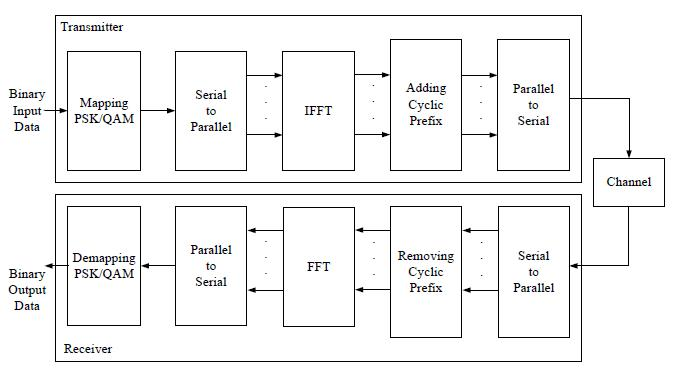
\includegraphics[width=12cm]{content/fig/basic_ofdm_design.JPG}
\label{fig:basic_ofdm}
\captionof{figure}{Basic baseband OFDM system}
\end{center}

In practice, to prevent sharp transactions at the sample time boundaries, a windowing block is used for filter shaping. In conclusion, spectrum utilization is enhanced dramatically. Therefore, the baseband OFDM symbol can be written as below:\\
\begin{equation} \label{ofdm_window}
\begin{split}
s_{k}(t)=
\left\{
	\begin{array}{ll}
	w(t - t_{s})\sum\limits_{i=-\frac{N}{2}}^{\frac{N}{2}-1} d_{i+\frac{N}{2}} \exp\lbrack j2\pi\frac{i}{T}(t- t_{s}- T{g}) , & t_{s}\le t < t_{s} + (1+\beta)T_{sym}\\
	0, & \mbox{otherwise}
	\end{array}
\right.
\end{split}
\end{equation}

where $T_{g}$ is the guard interval duration, $T_{sym}= T+ T_{g}$ is the OFDM symbol period,
symbol starting time $t_{s}= kT_{sym}$, and $w(t-t_{s})$ is the pulse shaping window, which is
usually a raised cosine filter, and $\beta$ is the roll-off factor.\\


\section{OFDM Specifications in IEEE 802.11a Standard}
\subsection{System Design}

In reality, having an anti-aliasing configuration, oversampling is performed before passing the digital signal to digital-to-analog converter. There are many other blocks in standards like channel coding, symbol interleaving and channel estimation.\\
In comparison to the fundamental architecture shown in Figure 000, some other building blocks are added in a practical IEEE 802.11 design shown in Fig 00, marked with blue and dashed on line. At the transmitter, several "null" subcarriers or tones are reserved besides of the data subcarriers in order to perform oversampling of the transmitted signal. In this context, "null" means the symbol carried on this subcarrier has a value of zero. Besides, some other subcarriers used as pilot for channel estimation are also inserted. The subcarriers are allocated at the input of the IFFT block to generate a phase shift. The windowing for pulse shaping is achieved after CP extension.\\

\begin{center}
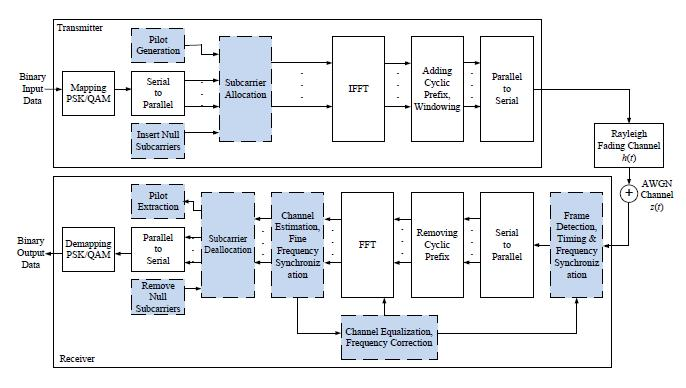
\includegraphics[width=12cm]{content/fig/ieee_system_design.JPG}
\captionof{figure}{Architecture of an OFDM system}
\end{center}

At the receiver side, the frame synchronization and detection for both timing and frequency is performed in the first stage. Channel estimation is performed after the FFT block outputs the preambles in the frequency domain. The result is fed back to the FFT block for the equalization, which eliminates the effects of fading channel, while the fine synchronization for both timing and frequency is also added to further improve the system performance.\\
At least these basic parameters should be specified for a system design:\\
1) Delay spread expected for the channel (300 ns)\\
2) Guard duration (800 ns) which describes symbol duration (4.0 $\mu$s)\\
3) Available bandwidth\\
4) Data rate\\

For indoor environment a delay spread less than 300 ns expected. We consider the guard duration 800 ns, which effectively protects the signal from ISI in the indoor environment and some of the outdoor wireless communication environments. Five times the guard duration for limiting the power and bandwidth loss is regarded for the symbol duration, and is set to 4.0 $\mu$s in our case. Hence, the OFDM symbol rate is 0.25 mega symbol per second (Mbaud).\\
Keep in mind, the useful OFDM symbol duration without the guard interval is 3.2 $\mu$s. So, the subcarrier spacing, which is the reciprocal of the useful symbol duration, can be determined as 312.5 kHz. Assuming that there is a bandwidth of 20 MHz available, the number of subcarriers is calculated to be 64. This is exactly the same as the specification defined in IEEE 802.11a standard.\\
As mentioned, some tones are reseved for pilot subcarries (channel estimation), null subcarriers (realizing oversampling to avoid aliasing) and windowing (reduce the out-of-band spectral energy).\\
In our design we chose 48 data tones and 4 pilot subcarriers. So, 52 subcarries are occupied. Applying a raised-cosine window with roll-off factor $\beta$= 0.02 the total occupied bandwidth is\\
\begin{center}
$(1+ 0.02)\times(52 \times 312.5kHz) \approx 16.6MHz$
\end{center}

To accomplish Oversampling, some zeros before and after the data vector are appended in the frequency domain as shown below.\\

\begin{center}
\includegraphics[width=12cm]{content/fig/oversample.JPG}
\end{center}

The nonzero data values are mapped onto the subcarriers around 0 Hz, and the zeros are mapped onto frequencies around sampling rate.

Basically, in the BPSK modulation is applied on each subcarrier, each symbol for an
individual subcarrier has one bits. The bit rate achieves without channel coding:\\
\begin{center}
$\frac{1}{4.0\mu s} \times 48 \times 1= 12Mbps$
\end{center}

The same calculation can be perform for QPSK to reach 24Mbps. But, channel coding will reduce this values. Variation of coding rates and modulation methods, In the 802.11a standard, the data rate ranges from 6 Mbps to 54 Mbps.\\

\begin{center}
\captionof{table}{System parameters defined for the proposed OFDM system}
\vspace{0.5cm}
\begin{tabular}{c|c|c}
Parameter&Description&Value\\ \hline
$B_{w}$&Available channel bandwidth&$20MHz$\\
$\sigma_{\tau}$&Delay spread of the channel& $<300 ns$\\
$T_{g}$&Guard interval duration&$0.8\mu s$\\
$T_{sym}$&OFDM symbol period&$4.0\mu s$\\
$T$&Effective symbol duration (FFT period)&$3.2\mu s (=T_{g}- T_{sym})$\\
$T$&Effective symbol duration (FFT period)&$3.2\mu s (=T_{g}- T_{sym})$\\
$\Delta f$&Subcarrier spacing&$312.5kHz (=1/T)$\\
$N_{g}$&Number of guard samples&$16$\\
$N$&FFT size&$64= B/\Delta f s$\\
$N_{d}$&Number of data subcarriers&$48$\\
$N_{p}$&Number of pilot sucarriers&$4$\\
$N_{u}$&Number of used subcarriers&$52$\\
$B_{u}$&Signal occupied bandwidth&$16.6MHz$\\
&Modulation type&$BPSK, QPSK$\\
$R_{b}$&Data rate without coding&$12Mbps, 24Mbps$\\
\end{tabular}
\end{center}

\subsection{IEEE 802.11a Standard in Time and Frequency}
A packet of OFDM will be described here. In an OFDM frame, a preamble which carries no data is transmitted first, followed by the signal field which give some information about data and transmitted data. As indicated in Figure 00, an OFDM frame has the general form as below:
\begin{center}
$s_{OFDM}(t)= s_{preamble}(t)+ s_{signal}(t- T_{preamble})+ s_{data}(t- T_{preamble}- T_{signal})$\\
\end{center}
where\\
\begin{center}
$s_{preamble}(t)= s_{short}(t)+ s_{long}(t- T_{short})$\\
\end{center}

The preamble starts with 10 short training symbols (STSs) from T1 to T10, followed by a guard interval (GI2) and two long training symbols (LTSs) L1 and L2. Both the short and long training sequences have an 8 $\mu$s duration and the entire preamble lasts for 16 $\mu$s. Then, a 3.2 $\mu$s signal symbol, as well as 800 ns guard interval is transmitted. This field bears some information necessary for the data symbols, such as the coding rate and length. Finally the various data symbols that carry user information are transmitted. Each data symbol has a duration of 4.0 $\mu$s, within which there is a 800 ns CP, as already described.\\
The application of STS and LTS for training are different. STS used for AGC, frame detection, coarse timing and frequency synchronization. Each symbol in this sequence has a duration of 800 ns and contains 16 samples, and is identical to one another.
 It will be shown in a professional system, auto-correlation will apply to this portion to perform such the operations. After the short training sequence is transmitted, a 1.6 $\mu$s guard interval that contains 32 samples is introduced. The LTS is cyclically extended within this interval. Then two identical LTSs with the same duration of 4.0 $\mu$s are followed. The LTS is used for fine frequency offset and channel estimation. It will be described that a cross-correlation with a stored array is done for extraction of the offset.\\



\begin{center}
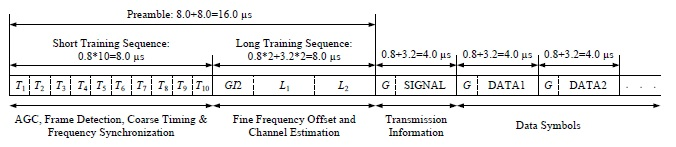
\includegraphics[width=12cm]{content/fig/ofdm_frame.JPG}
\end{center}

As we already analyzed, 52 subcarriers are used for an OFDM data symbol and pilot. Oversampling is achieved by adding 12 null subcarriers in order to eliminate aliasing which might occur during digital to analog conversion. Because FFT shift is performed, the null subcarriers with a value of zero are located in the middle of the input vector for the IFFT block. Note that dc carrier is not used to transmit data. The short and long training sequences can also be applied to this mapping rule, since they both have a length of 52 samples with frequency index from -26 to +26.\\


\section{Hardware Introduction}
\subsection{Processor}
\begin{center}
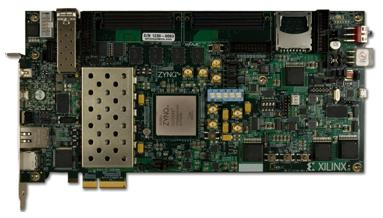
\includegraphics[width=12cm]{content/fig/ZC706.JPG}
\captionof{figure}{Xilinx Zynq-7000 SoC ZC706 Evaluation Kit}
\end{center}

\subsection{Radio Board}
\begin{center}
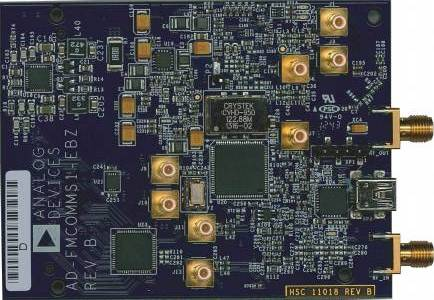
\includegraphics[width=10cm]{content/fig/fmcomms1.jpg}
\captionof{figure}{AD-FMCOMMS1-EBZ (Radio Board)}
\end{center}

\begin{center}
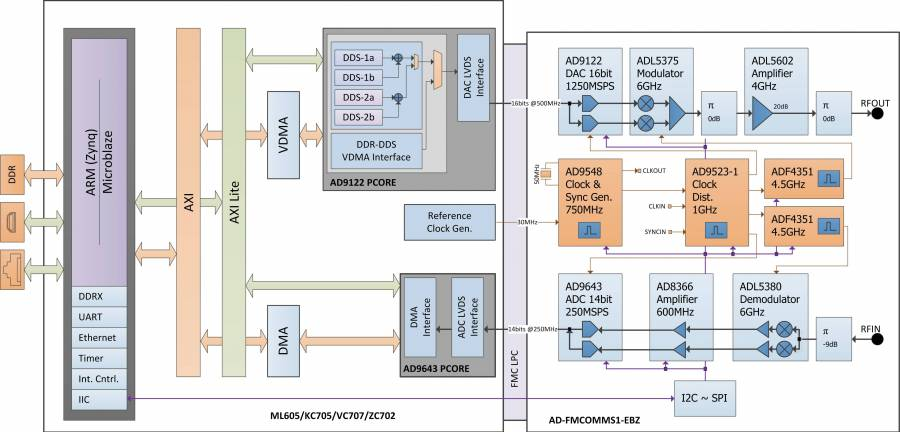
\includegraphics[width=15cm]{content/fig/fmcomms1Blockdiagram.jpg}
\captionof{figure}{AD-FMCOMMS1-EBZ Block Diagram}
\end{center}

\subsection{Clock Chain on FMCOMMS1}
Now, we discuss more about the clock chain and distribution mechanism on the board to find some meaningful number. As you can see in the figure, we configure the board and internal FPGA architecture to generate a 30MHz clock to the RF board. This 30MHz is just chosen because a relevant crystal mounted on the Zynq board and the all generated clock is supposed to be in-phased with it. This 30MHz is an input for AD9548 as a clock generator/synchronizer which has a very precise PLL inside to generate a 20MHz.\\
The AD9548 generates an output clock synchronized to one of up to four differential or eight single-ended external input references. The digital PLL allows for reduction of input time jitter or phase noise associated with the external references. The AD9548 continuously generates a clean (low jitter), valid output clock even when all references have failed by means of a digitally controlled loop and holdover circuitry. AD9548 is a very complicated device to generate 20MHz with maximum precision.\\

\begin{center}
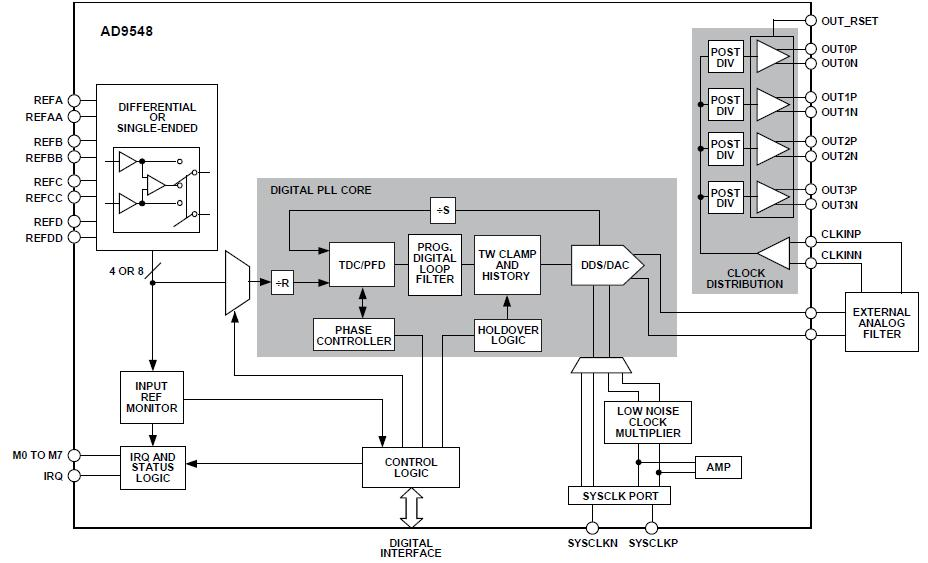
\includegraphics[width=15cm]{content/fig/ad9548BlockDiagram.JPG}
\captionof{figure}{AD9548 Block Diagram}
\end{center}

The next IC in the clock chain is AD9523-1 which is Low Jitter Clock Generator. The AD9523-1 provides a low power, multi-output, clock distribution function with low jitter performance, along with an on-chip PLL and VCO with two VCO dividers. The on-chip VCO tunes from 2.94 GHz to 3.1 GHz. The AD9523-1 is defined to support the clock requirements for
long term evolution (LTE) and multicarrier GSM base station designs. It relies on an external VCXO to provide the reference
jitter cleanup to achieve the restrictive low phase noise requirements necessary for acceptable data converter SNR performance.\\
The input receivers, oscillator, and zero delay receiver provide both single-ended and differential operation. When connected to a recovered system reference clock and a VCXO, the device generates 14 low noise outputs with a range of 1 MHz to 1 GHz, and one dedicated buffered output from the input PLL (PLL1). The frequency and phase of one clock output relative to another clock output can be varied by means of a divider phase select function that serves as a jitter-free, coarse timing adjustment in increments that are equal to half the period of the signal coming out of the VCO.\\
In  our chain we have a 80MHz VCXO connected to AD9523-1. It is supposed to generated 40MHz for ADC, DAC and also the main OFDM architecture FPGA program. You can see the specification of the crystal oscillator in ....\\

\begin{center}
\includegraphics[width=10cm]{content/fig/cvhd.JPG}
\captionof{figure}{CVHD-950 Ultra Low Phase Noise Oscillator}
\end{center}


\section{Expectations for CFO on FMCOMM1}

In implementation of an OFDM chain, we should have good understanding the range of carrier frequency offsets which can be expected on our hardware platform. Our RF board foundation is based on FMCOMMS1. As a result, the elements in term of phase -noise and CFO should be studied. The main RF frequency refrence is a Crystek CVHD-950 (VCXO). This VCXO provides a clock signal at a nominal frequency of 80 MHz. Actual output frequency varies as a function of multiple factors, and is only specified by the manufacturer with some tolerance. The CVHD-950 is specified with a frequency tolerance of $\pm$4 ppm. Thus, we must design for a reference frequency of 80$\pm$0.000320 MHz. Imagine our target RF carrier frequency is 2452 MHz which implies 2400 MHz$\pm$4 ppm (or 2400$\pm$0.009600 MHz).\\
The worst case CFO will occur when the transmit and receive nodes operate at opposite ends of this range. Thus, for operation in the 2.4 GHz band our OFDM transceiver design must be ready to handle any carrier frequency offset up to $\approx$20 kHz.


\section{Time Domain CFO Correction}
Prevention of the degradation of CFO, the receiver should estimate and correct the offset in the time domain before the FFT block. The FFT block translates the received signal into the frequency. Regarding to the variety issue of OFDM, many estimation algorithms have been proposed.\\

\section{System Analysis by Simulation}
\label{sec_anasim}

\section{Carrier Frequency Offsets}
\label{sec_simstruct}
As a result of the frequency variation between local oscillators of the transmitter and the receiver nodes that generate the carrier signals, carrier frequency offsets (CFO) is happened. It causes when the baseband signal is going to be translated to RF. The issue is understood well but the impact to overcome CFO and suppression this phenomena is always depend on the specific parameters of the given transceiver and the hardware.\\
The origin of the CFO effect is studied in this section. We explore in a specific scenario of OFDM and the impact on the hardware design. Both simulation and experiments will be demonstrated and the CFO estimation and compensation is described.\\

\subsection{Origin of CFO}
A simple model of a radio transmitter and receiver can depict the basis of the CFO source.

\begin{center}
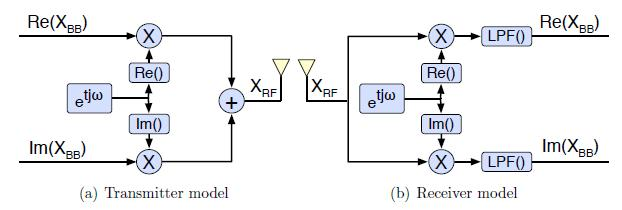
\includegraphics[width=\textwidth]{content/fig/cfo_radio_model.JPG}
\captionof{figure}{General models of a direct conversion RF}
\label{cfo_radio_model}
\end{center}

In Figure \ref{cfo_radio_model}, $\omega$ is The carrier frequency and $X_{BB}$ is the complex baseband signal, $X_{RF}$ is
a real-valued RF signal. These models simplified many other operations in a real RF transceivers although none of these affect the up/down-conversion processes as they relate to CFO.\\
These equations about transmit and receive processes can be written in equation (\ref{eq_tx_rx_process}):

\begin{equation}\label{eq_tx_rx_process}
\begin{split}
X_{RF} & = TX(X_{BB})\\
& = Re(X_{BB})\cos(\omega t) - Im(X_{BB})\sin(\omega t)\\
& = \frac{1}{2} (X_{BB} e^{jt\omega} + X^{*}_{BB} e^{-jt\omega})\\
\\
X_{BB} & = RX(X_{RF}, \omega)\\
& = LPF(X_{RF} e^{j\omega t})
\end{split}
\end{equation}


Assume a signal $S_{BB}$ transmitted with carrier frequency $\omega_{S}$ which is received with carrier frequency $\omega_{D}$. we can express the received baseband signal $D_{BB}$ in terms of the transmitted baseband signal $S_{BB}$ and the carrier frequencies. Then:\\

\begin{equation} \label{DBB_SBB}
\begin{split}
D_{BB} & = LPF(\frac{(S_{BB} e^{jt\omega_{S}} + S^{*}_{BB} e^{-jt\omega_{S}})e^{jt\omega_{D}}}{2})\\
&= S_{BB}(e^{jt(\omega_{S}- \omega_{D})})
\end{split}
\end{equation}

The received baseband signal is equal to the original baseband signal modulated by a complex sinusoid. In the frequency domain, this gives a received spectrum equal to the transmitted one, only shifted away from DC by the difference in the carrier frequencies of the transmitter and receiver (i.e. $\omega_{S}- \omega_{D}$). This shift of the received
signal is the baseband manifestation of carrier frequency offset.

\subsection{Impact of CFO}
\label{Impact_of_CFO}
There are two destructive impacts on an OFDM system. Firstly, the phase offset across subcarriers in an symbol which can be  estimated and corrected in frequency domain to prevent errors in a constant rotated constellation. Some subcarriers are allocated as pilot tones which receiver can estimate phase errors.\\
The second effect of CFO is the degradation of orthogonality between subcarriers in receiver's FFT which causes inter-carrier interference (ICI). ICI acts an effective SNR reduction as a result of CFO increasing. [...]\\
The impact is displayed in Figure \ref{cfo_impact_on_ici} which is shown simulated OFDM system uses 10 MHz bandwidth and 64 subcarriers, 48 of on a random 16-QAM data symbols. CFO and AWGN are applied between the transmitter and receiver. The receiver model uses perfect knowledge of the CFO to correct the phase offset in each OFDM symbol, but does not implement any correction for ICI.\\

\begin{center}
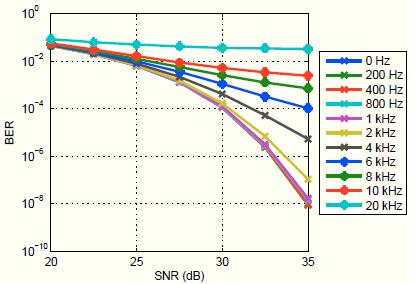
\includegraphics[width=\textwidth]{content/fig/cfo_on_ici.JPG}
\captionof{figure}{OFDM performance loss due to CFO-induced ICI.}
\label{cfo_impact_on_ici}
\end{center}

The results shows that for large CFOs errors caused by ICI dominate performance, even at high SNR. It is also
clear that for small CFOs performance is dominated by SNR. Specifically, for frequency offsets smaller than 1 kHz, the
performance degradation due to ICI is negligible.\\


